\documentclass[11pt,a4paper]{article}

\usepackage[utf8]{inputenc}
\usepackage[spanish]{babel}

\usepackage{enumitem}

\usepackage{cite}

\usepackage{url}
\usepackage[hidelinks]{hyperref}

\usepackage{graphicx}
\usepackage{color}

\bibliographystyle{plain}

\title{Análisis del \emph{malware MiniDuke}}

\author{\begin{tabular}[center]{c}
          Ignacio Ballesteros González \\
          \small w140062 \\
          \small 05448027V \\
        \end{tabular}
      }

\date{\today}

\begin{document}

\maketitle
\tableofcontents
\normalsize
\begin{abstract}
  Segunda práctica de la asignatura de \emph{Seguridad de las
    Tecnologías de la Información}. Se realizará el estudio de una
  muestra del código malicioso \emph{MiniDuke}. Se ha elegido la
  opción \textit{(c)} de estudio en base a las normas establecidas.

  \begin{center}
    $1 + ((5448027 * 726391632)~mod~330) = 175$
  \end{center}
\end{abstract}

\section{Introducción}
\label{sec:intro}
\emph{MiniDuke} es un malware que utiliza un \emph{exploit 0-day} de Adobe
Reader para lograr acceso a la máquina objetivo. El término de
\emph{MiniDuke} también se aplica a la campaña que usaba esta
herramienta, enmarcada en una operación de espionaje a gobiernos. \cite{Dukes}

\begin{description}[leftmargin=9em,style=nextline]
  \item[Código malicioso] \emph{MiniDuke}
  \item[Tipo] No autorreplicante
  \item[Familia] Exfiltración, \emph{Spyware, Backdoor, APT}
\end{description}

\section{Ficha resumen}

\begin{description}[leftmargin=5.5em,align=right,labelwidth=2cm]
\item[Denominación] MiniDuke
\item[Origen/autor] The Dukes (Rusia)\footnote{Atribución no del todo clara. Basada en las suposiciones del grupo investigador \emph{F-Secure}.}\cite[p.~26]{Dukes}
\item[Destinatario] Instituciones gubernamentales y
  afiliadas. \cite[p.~18]{Kaspersky}\\
  \begin{tabular}{l |l}
    \textbf{País}&\textbf{Red} \\ \hline
    Ucrania&Gobierno, Empresas privadas \\
    Bélgifa&Embajada / Gobierno \\
    Portugal&Gobierno \\
    Rumanía&Gobierno \\ 
    Irlanda&Gobierno \\
    Estados Unidos& \emph{Think tank(s)}, Sistema de Salud \\
    Hungría&Social foundation
  \end{tabular}
  
\item[Fecha de lazamiento] \emph{Loader}\footnote{Parte de MiniDuke
    fue usado antes por otro malware, \emph{PinchDuke}, pero aquí se
    le llamará \emph{loader}}: julio de 2010. \emph{Backdoor}: mayo de 2011.
\item[Fecha de descubrimiento] 27 de febrero de 2013\cite{Crysys13}
\item[Tipo de código malicioso] \emph{downloader, backdoor}, exfiltración.

  \begin{center}
    \textbf{Funcionamiento general}
  \end{center}
  
\item[Modo de infección] El vector de infección que se ha encontrado
  ha sido mediante \emph{ingeniería social} con la infección de
  \emph{PDFs} en \emph{emails}. La vulnerabilidad utilizada fue un
  \emph{0-day}\footnote{Vulnerabilidad no conocida hasta el momento
    del descubrimiento del \emph{malware} que la explota.} de Adobe
  Reader\footnote{Adobe Reader y Acrobat 9.x anterior a
    9.5.4, 10.x anterior a 10.1.6, y 11.x anterior a 11.0.02} y Acrobat. \cite{Bitdefender13}\\
  \begin{tabular}[h]{l l}
    2012 & CVE-2011-2462 \\
    2013 & CVE-2013-0640           
  \end{tabular}
\item[Modo de replicación] No aplica.
\item[Modo de propagación] Campañas de \emph{phising}.
\item[Modo de ocultación] Uso de vulnerabilidas no conocidas
  (\emph{0-day}). Comunicación con el exterior mediante \emph{IPs}
  fiables (\emph{Twitter, Google}) para pasar desapercibido en la
  exfiltración. Compresión del código del
  \emph{payload}. \cite[p.~5]{Kaspersky}
\item[Ejecución de la carga] Usa el mismo \emph{payload} que
  \emph{Itaduke}. Código \emph{JavaScript} comprimido que detecta el
  \emph{PDF} de infección y crea un fichero temporal de
  instalación. Posteriormente pasa a ejecutar un \emph{dropper}
  específico para las características del ordenador de la víctima.\cite{Kaspersky}
\end{description}

\paragraph{Tiempo de vulnerabilidad relacionada}~\\\\\qquad Según los
últimos datos, el \emph{loader} de \emph{MiniDuke} se ha utilizado
desde 2010 hasta 2015. \cite{Dukes} En la figura \ref{fig:timeline}
(en \textcolor{cyan}{azul}) se puede ver el periodo de actividad
comparado con el resto de \emph{malware} de su familia.

\begin{figure}[h]
  \centering
  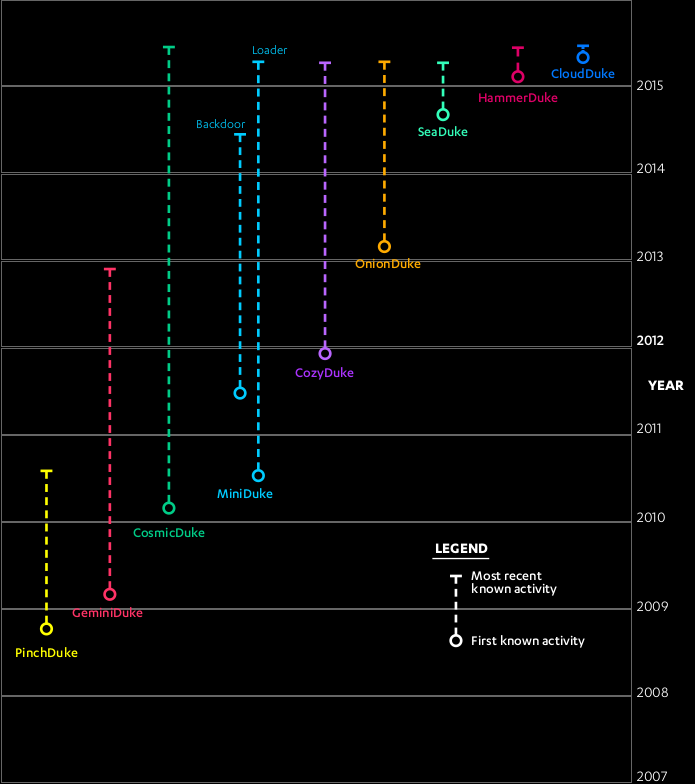
\includegraphics[width=\textwidth]{./referencias/timeline.png}
  \caption[Linea temporal \emph{Dukes}.]{Linea temporal de varias
    herramientas de la familia \emph{Duke}.}
  \label{fig:timeline}
\end{figure}

\paragraph{Modo de desinfección}
\paragraph{Ejemplo de ataque donde se ha empleado}
\paragraph{Medidas de seguridad tomadas tras su descubrimiento}
\paragraph{Resto de miembros de su familia}
\paragraph{Otra información relevante}

\section{Conclusiones}
\label{sec:conclusiones}

\bibliography{malware}

\end{document}
